\section{Background}
Here we will dicuss the background of the problem, where code quality can be used, what are the benefits to using it and how 
can we create a similar tool.
\subsection{Applicability to Industry}
Where we start to move towards ensuring more quality in our written code is when developing code in Industry,
many techniques are utilised which includes the use of code review.
\subsubsection{Code Review}
Manual code review is described as peers reviewing the code that has been written to look for problems within the written code,
the results of this can be staggering on the outcomes of delivered software.
In their 2006 book Jason Cohen describes the outcome of a company after implementing code review for only 3 months. \cite{cohen2006best}
\begin{verbatim}
The result: Code review would have saved half the cost of
fixing the bugs. Plus they would have found 162 
additional bugs.
\end{verbatim}
This shows the incredible power of having another pair of eyes on code before it is shipped,
not only to reduce bugs as previously stated but to transfer knowledge, increase team awareness and create alternative solutions to problems \cite{modernCodeReview}


\subsubsection{Use of tools in Code Review}
As we have shown that code review is an important and effective task for creating quality software, we must understand the limitations it has.
One of the biggest problems with Code Reviews is how long they can take
the use of code quality tools speeds up the code review process by identifying potential problem areas in the code. \cite{confusionInCodeReviews}
\newline
The automatic detection and amending of simple errors in code is said to allow for developers to utilise code review for deeper and more subtle issues. \cite{modernCodeReview}
\begin{verbatim}
Code review is fertile ground to have an impact with 
code analysis tools.
\end{verbatim}\cite{modernCodeReview}




\subsection{Static Analysis}
In this project the student will focus on Static Analysis methods which are performed on source code this
is as opposed to Dynamic Analysis which is the analysis of the properties of a running program \cite{dynamicAnalysis}
\subsubsection{\textbf{Cyclomatic Complexity (CC)}}
is defined as
\begin{verbatim}
The number of linearly independent paths within a 
piece of code
\end{verbatim}
The piece of code in figure \RefFig{fig:simple-func1} has a CC of 1.
\begin{figure}[h]
    \begin{lstlisting}[language=Javascript]
function test(a){
    return a
}
        \end{lstlisting}
    \caption{Javascript example of very simple function}
    \Description{Javascript example of very simple function}
    \label{fig:simple-func1}
\end{figure}
So does Figure \RefFig{fig:simple-func2}.
\begin{figure}[h]
    \begin{lstlisting}[language=Javascript]
function test(a){
    let b = a
    b = a*b
    b*=42
    return b
}
        \end{lstlisting}
    \caption{Javascript example of less simple function}
    \Description{Javascript example of less simple function}
    \label{fig:simple-func2}
\end{figure}
When we add a control statement with 2 paths our control flow graph now contains 2 possible flows which gives us a CC of 2 as shown in Figure \RefFig{fig:complex-func}.
\begin{figure}[h]
    \begin{lstlisting}[language=Javascript]
function test(a,b){
    if(a>2){
        return a
    }
    return b
}
        \end{lstlisting}
    \caption{Javascript example of more complex function}
    \Description{Javascript example of more complex function}
    \label{fig:complex-func}
\end{figure}
\newline
CC is computed by evaluating the Control Flow Graph (CFG) of a program.
\newline
It can be calculated as
\newline
\begin{verbatim}
    CC = E - N + 2p
\end{verbatim}
Where E = Edges , N = Nodes and p = connected components (which is always one for an independent function) \cite{cycloMaticComplexity}. Therefore the code in Figure \RefFig{fig:cfgcode} is:
\begin{verbatim}
    CC = 4 - 4 + 2
    CC = 2
\end{verbatim}
Which we can also see from following the graph itself.
\begin{figure}[h]
    \begin{lstlisting}[language=Javascript]
function test(a,b){
    if (a < 10){
        a++;
    }else{
        a--;
    }
    return a
}
                \end{lstlisting}
    \caption{Simple Javascript function with control statements}
    \Description{Simple Javascript function with control statements}
    \label{fig:cfgcode}
\end{figure}
\begin{figure}[h]
    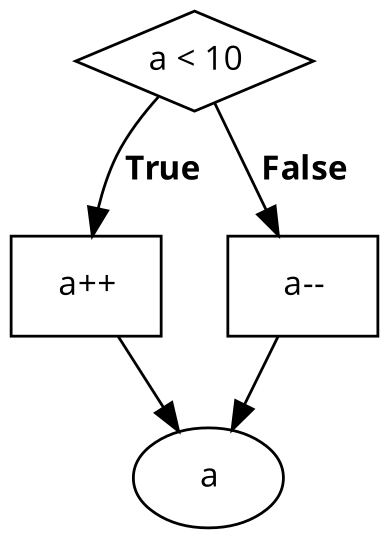
\includegraphics[width=.2\textwidth]{appendix/A/AppendixA.png}
    \caption{Control Flow Graph from code sample in \RefFig{fig:cfgcode} created using code2flow \cite{code2flow} see Appendix A}
    \Description{Control Flow Graph of code }
    \label{fig:cfg}
\end{figure}

CC can be an excellent measure to follow as not only does it make us segment our code for readability and extendability it ensures there are not too many test cases for a function.
\newline
McCabe suggested this in his 1976 paper \cite{cycloMaticComplexity}
\begin{verbatim}
"Programmers have been required to calculate complexity 
as they create software modules. When the complexity 
exceeded 10 they had to either recognize and modularize 
subfunctions or redo the software. The intention was to 
keep the "size" of the modules manageable and allow for 
testing all the independent paths..."
\end{verbatim}
Since it's publication there have been various critiques of the metric, the main one being it's correlation with
Source Lines Of Code. On a given piece of code SLOC will linearly track CC, proven in a study of over 1.2 million files of source code \cite{graylin2009cyclomatic}.
While this being the case, the study also found that although LOC has massive predictive power to follow CC in a source code file, there are outliers
which caused variance within the study.
The relationship between CC and SLOC has been further analysed in a 2014 study, the study posits that this variation becomes more apparent
when SLOC increase, control flow statements do no linearly increase with SLOC \cite{CCANDSLOC}.
\begin{verbatim}
    "...there is no evidence of a strong
    linear correlation between SLOC and CC in this large 
    corpus. Suggesting that for Java methods CC measures 
    a different aspect of source code than SLOC..."
    \end{verbatim}
\cite{CCANDSLOC}
Also as CC describes the amount of tests that a piece of software requires it still has it's use in Code Quality analysis.


\subsubsection{\textbf{Halstead Complexity}}
In his 1977 book M.H. Halstead described a set of complexity measures. \cite{HalsteadComplexity}
\newline
These are described as such for any software program.
\begin{itemize}
    \item n\textsuperscript{1} : the number of unique operators
    \item n\textsuperscript{2} : the number of unique operands
    \item N\textsuperscript{1} : the total number of operators
    \item N\textsuperscript{2} : the total number of operands
\end{itemize}
Then several measures can be calculated from these.
\begin{itemize}
    \item Program Vocabulary    : n = n\textsuperscript{1} + n\textsuperscript{2}
    \item Program length        : N = N\textsuperscript{1} + N\textsuperscript{2}
    \item Calculated estimated program length : \newline \^{N} = n\textsuperscript{1} log \textsubscript{2} n\textsuperscript{1} + n\textsuperscript{2} log \textsubscript{2} n\textsuperscript{2}
    \item Volume                : V = N * log \textsubscript{2} n
    \item Difficulty            : D =  $\textfrac{n\textsuperscript{1}}{2}$ * $\textfrac{N\textsuperscript{1}}{n\textsuperscript{1}}$
    \item Effort                : D * V
    \item Time required to program : T = $\textfrac{E}{18}$
    \item Number of delivered bugs : B = $\textfrac{V}{3000}$
\end{itemize}

Example taken from \textit{Eindhoven University of Technology} \cite{softwareEvolution}
\begin{verbatim}
        main()
        {
            int a, b, c, avg;
            scanf("%d %d %d", &a, &b, &c);
            avg = (a+b+c)/3;
            printf("avg = %d", avg);
        }
    \end{verbatim}
In this example c program
\begin{itemize}
    \item n\textsuperscript{1} : 12
    \item n\textsuperscript{2} : 7
    \item n : 19
    \item N\textsuperscript{1} : 27
    \item N\textsuperscript{2} : 15
    \item N : 42
    \item \^{N} : 12 log \textsubscript{2} 12 + 7 log \textsubscript{2} 7 = 62.67
    \item V : 42 * log \textsubscript{2} 19 = 178.4
    \item D : $\textfrac{12}{2}$ * $\textfrac{15}{7}$ = 12.85
    \item E : 12.85 * 178.4 = 2292.44
    \item T : $\textfrac{2292.44}{18}$ = 127.357 seconds
    \item B : $\textfrac{178.4}{3000}$ = 0.059
\end{itemize}


\subsubsection{\textbf{Chidamber and Kemerer Class Design Metrics}}
A metric used in languages with OOP features is the Chidamber and Kemerer metrics \cite{classDesignMetrics}.
These metrics are used to determine the complexity of classes and their methods.

\textbf{Weighted Methods per Class (WMC)}
This describes the number of methods per class, a high WMC count has been found to lead to more problems in the code.
Classes with a high WMC could point to being needed to be split into multiple smaller classes.

\textbf{Depth of Inheritance Tree (DIT)}
This describes the depth of the inheritance of a class.
\begin{figure}[h]
    \begin{lstlisting}[language=Javascript]
class animal{
    constructor(){
        this.isAnimal = true;
    }
}

class dog extends animal{
    constructor(){
        super()
        this.isDog = true;
    }
}

class pug extends dog{
    constructor(){
        super()
         
    }
}
                \end{lstlisting}
    \caption{Example JavaScript classes with inheritance}
    \Description{Example JavaScript classes with inheritance}
    \label{fig:DIT}
\end{figure}

In Figure \RefFig{fig:DIT} we have a few example classes, the DIT values for these classes are as such.

\begin{verbatim}
    animal = 0
    dog = 1
    pug = 2
\end{verbatim}

It is recommended to have a DIT of 5 or less. \cite{classDesignMetrics}

\subsubsection{\textbf{Other Metrics}}
There are other metrics described Generally as Code Smells as described in Clean Code: A Handbook of Agile Software Craftsmanship \cite{cleanCode}.

\textbf{Function Lines}
This is a metric that is tied to the number of lines that can fit on a screen, it is suggestive of bad function design if a function cannot
fit on the screen, with the typical number of lines used being 20.

\textbf{Function Parameters}
A function with too many parameters suggests the need for the function to be split into smaller functions or the use of a parameter object
to allow for parameter specification in the function call.
\begin{verbatim}
"The ideal number of arguments for a function is
zero (niladic). Next comes one (monadic), followed
closely by two (dyadic). Three arguments (triadic)
should be avoided where possible. More than three
(polyadic) requires very special justification—and
then shouldn’t be used anyway"
\end{verbatim} \cite{cleanCode}

\textbf{Function / Class Redefinition}
This is quite self explanatory, it is usually bad practice to define the same function and/or class twice.

\textbf{Self Inheritance}
Another self explanatory measure, a class inheriting from itself would be redundant and possibly syntax breaking in many languages.


\subsubsection{\textbf{Problems with metrics}}
While considering these metrics it is important to remember the problems associated with them. Not only the critiques (as previously discussed) 
but also that written software source code is hard to purely quantify. 
Therefore it is important to ensure that metrics are used as an indication of a possible problem and not as evidence of a 
problem in it's entirety.
\newline
\begin{figure}[h]
    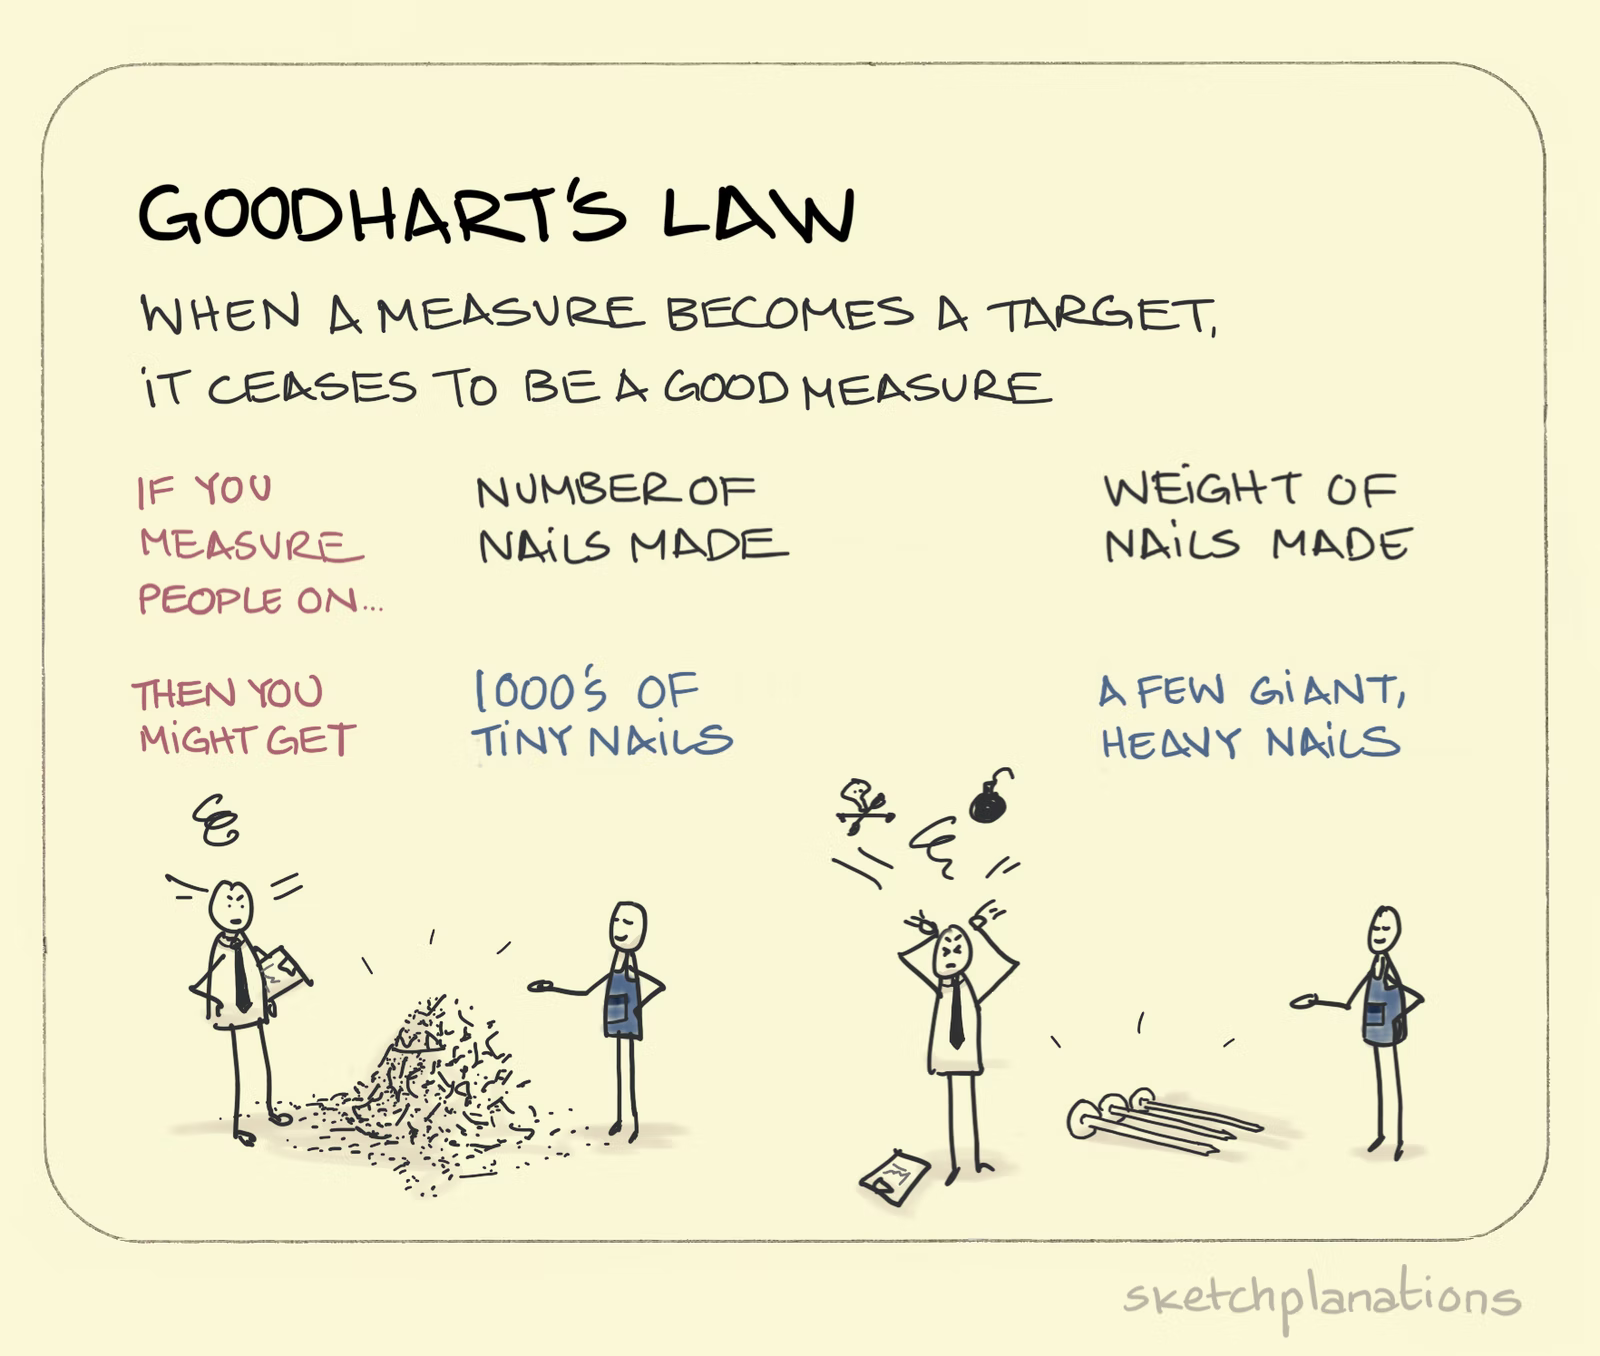
\includegraphics[width=.4\textwidth]{images/goodhart.png}
    \caption{Goodhart's Law Comic from Sketch Plantations \cite{sketchplanations}}
    \Description{Goodhart's Law Comic from Sketch Plantations  }
    \label{fig:goodhart}
\end{figure}
One way to understand this is Goodhart's law \cite{Goodhart1984}, first described to say:
\begin{verbatim}
    "Any observed statistical regularity 
    will tend to collapse once pressure is 
    placed upon it for control purposes"
\end{verbatim}
\cite{Goodhart1984}
Which was generalised by Marilyn Strathern to be:
\begin{verbatim}
    "When a measure becomes a target, 
    it ceases to be a good measure"
\end{verbatim}
\cite{strathern1997improving}
This is to say that when we use a statistic or a metric as the pure evaluation of a system, the person or organisation trying to fit the metric will 
seek to improve their score on the metric to the detriment of the overall system as emblematized by Figure \RefFig{fig:goodhart}.
\newline
While Goodhart used this to describe the Monetary Policy in the United Kingdom, it has been used in various situations such as 
Automotive Carbon Emissions, Individual Productivity in Software Engineering and Ratings in the British University system 
just to name a few \cite{NBERw22911} \cite{FRITZ201667} \cite{strathern1997improving}.


\subsubsection{\textbf{Social and ethical consdierations with research}}
A 
\newline problem with the research into metrics on code quality is the collection of source code to analyse, the data collected has 2 primary sources, 
Companies providing their software to researchers and use of Open Sourced Repositories. Both of these have problems associated with them. 
Companies have an incentive to want their software to be seen as superior to their competitors, this means that a company is likely to share cherry picked code 
that that consider to be of good quality, skewing the data. Open source repositories have a different and more 
ethical concern, is that participation in Open Source communities is skewed towards the perspectives of Male programmers in the age category of 
25-34 \cite{openSourcePerspective} \cite{womenInOpenSource}.
\begin{figure}[h]
    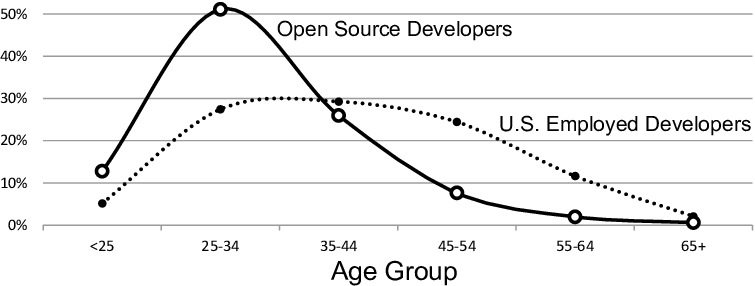
\includegraphics[width=.4\textwidth]{images/Age-distribution-for-open-source-and-general-developers.png}
    \caption{Graph showing Differing ages between \newline Open Source Developers and Employed Developers \cite{openSourcePerspective}}
    \Description{Graph showing Differing ages between Open Source Developers and Employed Developers}
    \label{fig:ageOpenSource}
\end{figure}

\subsection{Existing Code Quality Tools}
There are many tools used by the modern developer to increase the quality of their code, as shown these are important to be used in industry, but should 
also be used in education \cite{codeQualityEducation} \cite{codeQualityStudents}.
\subsubsection{\textbf{AST Explorer}}
AST explorer is a web application that allows you to view the JSON representation of the Abstract Syntax Tree (AST) of a language, it supports over 20 languages and 
up to 20 parsers for a given language. It also has the ability depending on the parser used to suggest readability and code styling fixes \cite{astexplorer}.
\subsubsection{\textbf{Clang Suite}}
Clang is a compiler capable of compiling c++ code, it has various tools associated with it for ensuring code quality.
One of the most popular and widely used throughout industry is Clang Tidy \cite{clangTidy}. Clang Tidy is a command line tool that can 
check for finding typical programming errors and readability, it also can use Clang Static Analyzer \cite{clangStatic} to preform control 
flow analysis.
\subsubsection{\textbf{ESLint}}
ESLint is a static analyser that can be built into an Integrated development environment \cite{wiki:Integrated_development_environment} 
or used as part of a Continuous Integration pipeline \cite{wiki:Continuous_integration}. The problems that ESLint looks for can be customised and 
it can be configured to automatically fix issues it encounters \cite{eslint}.


\subsection{Parsing}
In order to perform static code quality analysis we must parse the language, this is similar to a compiler in the beginning stages 
as shown in Figure \RefFig{fig:codeanalyser} and Figure \RefFig{fig:compiler}.
\begin{figure}[h]
    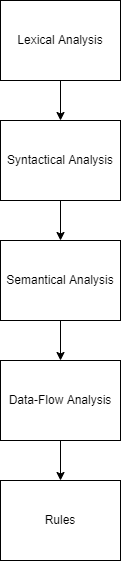
\includegraphics[width=.11\textwidth]{appendix/B/CodeAnalyser.png}
    \caption{Flow Diagram of stages of code analyser See Appendix B}
    \Description{Flow Diagram of stages of code analyser}
    \label{fig:codeanalyser}
\end{figure}
\begin{figure}[h]
    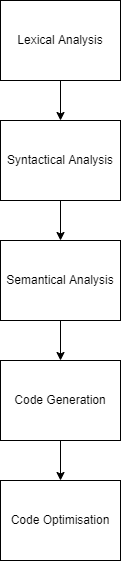
\includegraphics[width=.11\textwidth]{appendix/C/compiler.png}
    \caption{Flow Diagram of stages of a compiler See Appendix A}
    \Description{Flow Diagram of stages of a compiler}
    \label{fig:compiler}
\end{figure}
A parser takes input data, in our case Source Code, as text and builds a Data Structure, in our case an Abstract Syntax Tree (ABS) that represents 
the structure of the input. 
\subsubsection{\textbf{Automatic Parsing}}
A parser can be written by hand or can be generated by a parser generator, this is what we call Automatic Parsing or Semi-Automatic Parsing. 
An example of a Parser Generator is Nearley.js\cite{nearley.js} which implements the Earley Parsing Algorithm \cite{earley}.
\label{section:bnf}
Parser Generators typically take a definition of the language, the most common format of which is Backus-Naur-Form (BNF). 
BNF is what we call a meta language 
this is because it is a language that describes the syntax of another language, in this case a programming language. In the case of the example shown in Figure \RefFig{fig:bnf-emca} 
a "CommonToken" can be many different things, of these it can be an "IdentifierName" which can either be an "IdentifierStart" or two tokens together in the form of "IdentifierName" and "IdentifierPart"
\cite{bnf}.
\begin{figure}[h]
\begin{verbatim}
CommonToken::
    IdentifierName
    Punctuator
    NumericLiteral
    StringLiteral
    Template
        
IdentifierName::
    IdentifierStart
    IdentifierName IdentifierPart
        \end{verbatim}
    \caption{BNF grammar example in the form of an Excerpt from the ecmascript grammar definition \cite{ecmascript2017}}
    \Description{BNF grammar example in the form of an Excerpt from the ecmascript grammar definition}
    \label{fig:bnf-emca}
\end{figure}
\subsubsection{\textbf{Manual Parsing}}
If we don't want to use a parser generator we can write the parser ourselves, there are a few distinctions between the different 
methods of parsing that it is important to be aware of.

\paragraph{Top-down vs Bottom-up. } A Top-Down parser works from the top of the parse tree and works down to the lowest element (or leaf). A Bottom-Up Parser is the opposite of this 
which starts from the lowest leaf and works it's way up to the top of the parse tree. Bottom-up parsers tends to use right most derivation and Top-down parsers tend to use left most derivation, meaning that when evaluating nodes the right or left child of the current node is chosen. 
The difference is shown in a top down parsing manner between left and right most derivation in Figure \RefFig{fig:leftdir} and Figure \RefFig{fig:rightdir} \cite{topDownBottomUp}. 
\begin{figure}[h]
    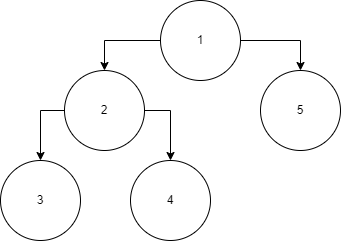
\includegraphics[width=.4\textwidth]{appendix/L/Leftmostderivation.png}
    \caption{Top Down Left Most Derivation of Parse Tree Diagram See Appendix L}
    \Description{Top Down Left Most Derivation of Parse Tree Diagram See Appendix L}
    \label{fig:leftdir}
\end{figure}
\begin{figure}[h]
    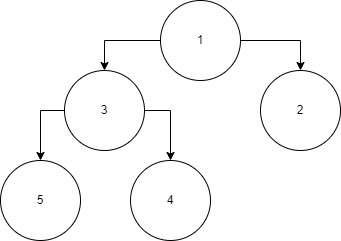
\includegraphics[width=.4\textwidth]{appendix/M/RightMostDerivation.png}
    \caption{Top Down Right Most Derivation of Parse Tree Diagram See Appendix M}
    \Description{Top Down Right Most Derivation of Parse Tree Diagram See Appendix M}
    \label{fig:rightdir}
\end{figure}

\paragraph{Recursive Descent.}
In section \RefFig{section:bnf} we discussed the grammar of a parser, a Recursive Descent Parser mimics this grammar in it's implementation , 
this will be shown later on in the report in the development section.
\paragraph{Predictive Parsing.} Another feature of parsing is Backtracking, in certain parsers , possibilities for the correct parse are evaluated and abandoned. Although with 
smart creation of grammar it is possible to use a lookahead to the next token to predict what to parse \cite{practicalCompiler}.


\subsubsection{Abstract Syntax Tree.}
\begin{figure}[h]
    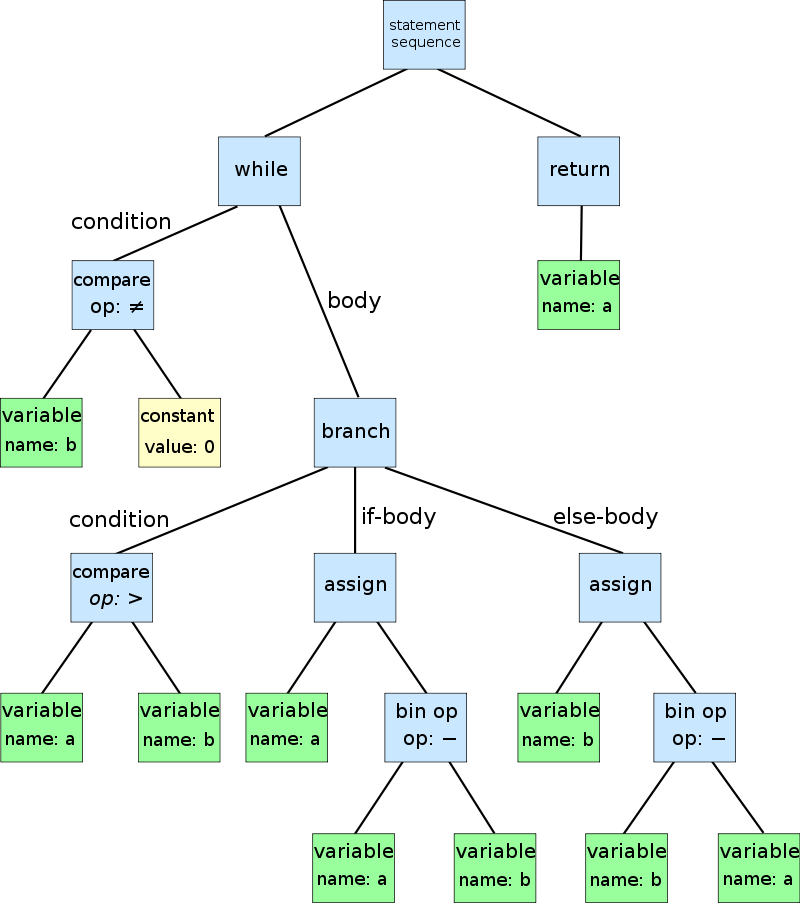
\includegraphics[width=.2\textwidth]{images/abstract-syntax-tree.png}
    \caption{Abstract Syntax Tree of Euclidean Algorithm \cite{astwiki}}
    \Description{graphical representation of abs of euclid algorithm}
    \label{fig:abs}
\end{figure}
Whatever parsing methodology we use, we need to create an AST this in an Abstract Syntax Tree. We can then use this representation of the code to preform our analysis.
The below code has been transformed into the AST in Figure \RefFig{fig:abs}
\begin{figure}[h]
    \begin{lstlisting}[language=Javascript]
        while(b != 0){
            if(a > b){
                a = a - b
            }else{
                b = b -a 
            }
        }
        return a
        \end{lstlisting}
    \caption{Javascript example of euclid's algorithm}
    \Description{Javascript example of euclid's algorithm}
    \label{fig:euclid}
\end{figure}

\subsection{Legal issues relating to Software Quality}
As the world of software development progresses and the measurement of code quality becomes standard practice 
ensuring high quality software can become a criminal liability. It could be argued that it is negligence to not use 
such a common practice as Code Quality analysis in the checking for bugs. Under the Tort Theory of Negligence. \cite{legalLiability}

\begin{verbatim}
"...responsibility is limited to only harmful defects
that could have been detected and corrected through 
“reasonable” software practices." 
\end{verbatim} \cite{legalLiability}.
Therefore if a defect in the software was to cause harm to someone, and that bug could have been found via the use of Code Quality Analysis 
,the person or organisation could be liable.

\subsection{Summary}
In summary, we have seen that Code Quality Analysis and the tools used to perform it , is and are valuable software development practices. Not only in 
the monetary sense but in the learning it can convey and facilitate. We have seen the types of metrics Code Quality can measure and discussed the 
critiques and rebuttals, not only to the metrics themselves but to following a metric in itself. We have discussed some of the various tools used 
and the development patterns used to construct them.
\newline
It is now time to implement such a system, to understand it from a deeper level and to produce an artifact that would provide value to end users.




